\section{Задача №3}
\textbf{Постановка задачи}:
Сформулировать и решить задачу Дирихле для уравнения Лапласа в прямоугольнике $l_{1} \times l_{2}$, когда заданы граничные условия $u(0, y) = \sin \left( {\dfrac{\pi y}{l_{2}}} \right)$, $u(l_{1}, y) = \sin \left( {\dfrac{\pi y}{l_{2}}} \right)$, а на остальных границах --- нулевые значения.

\textbf{Решение}:
Сформулируем задачу:
$$
\begin{cases}
\Delta u = 0,&\text{$x\in(0;l_{1}), y \in (0, l_{2})$}\\
u(0, y) = \sin{\dfrac{\pi y}{l_{2}}},&\text{$y\in[0;l_{2}]$;}\\
u(l_{1}, y) = \sin{\dfrac{\pi y}{l_{2}}},&\text{$y\in[0;l_{2}]$;}\\
u(x, 0) = 0,&\text{$x\in[0;l_{1}]$;}\\
u(x, l_{2}) = 0,&\text{$x\in[0;l_{1}]$.}
\end{cases}
$$

$$u = u(x, y)$$

Решение будем искать в виде:
$$ u = \sum_{n=1}^{\infty} c_{n} u_{n}^{(r)}, \text{где $u_{n}^{(r)} = X_{n}(x) Y_{n}(y)$}$$

Тогда:
$$ X''y + Y''X = 0 $$

$$ \dfrac{X''}{X} = -\dfrac{Y''}{Y} = \lambda_{n}$$

$$
\begin{cases}
Y'' + \lambda_{n}Y = 0\\
Y(0) = 0\\
Y(l_{2}) = 0
\end{cases}
\Rightarrow Y_{n}(y) = A \sin{\dfrac{\pi ny}{l_{2}}}, \lambda_{n} = \left( \dfrac{\pi n}{l_{2}} \right)^{2}, n = 1, 2, \ldots
$$

$$ X'' - \lambda_{n}X = 0$$

$$ X(x) = \tilde{A}e^{-\sqrt{\lambda_{n}}x} + \tilde{B}e^{\sqrt{\lambda_{n}}x}$$

Выберем другую ФСР в виде:
$$ X(x) = \{ \dfrac{\sh \sqrt{\lambda_{n}}x}{\sh \sqrt{\lambda_{n}}l_{1}}, \dfrac{\sh \sqrt{\lambda_{n}}(l_{1} - x)}{\sh \sqrt{\lambda_{n}}l_{1}} \}$$

$$ u(x, y) = \sum_{n=1}^{\infty} \sin{\dfrac{\pi n y}{l_{2}}} \left( \tilde{\tilde{A_{n}}} \dfrac{\sh{\dfrac{\pi n x}{l_{2}}}}{\sh{\dfrac{\pi n l_{1}}{l_{2}}}} + \tilde{\tilde{B_{n}}} \dfrac{\sh{\dfrac{\pi n (l_{1} - x)}{l_{2}}}}{\sh{\dfrac{\pi n l_{1}}{l_{2}}}} \right) $$

При $x = 0$:
$$ \sin{\dfrac{\pi y}{l_{2}}} = \sum_{n=1}^{\infty} \tilde{\tilde{B_{n}}} \sin{\dfrac{\pi ny}{l_{2}}}$$

$$\Rightarrow \tilde{\tilde{B_{n}}} = 0, \forall n \neq 1, \tilde{\tilde{B_{1}}} = 1$$

При $x = l_{1}$:
$$ \sin{\dfrac{\pi y}{l_{2}}} = \sum_{n=1}^{\infty} \tilde{\tilde{A_{n}}} \sin{\dfrac{\pi ny}{l_{2}}}$$

$$\Rightarrow \tilde{\tilde{A_{n}}} = 0, \forall n \neq 1, \tilde{\tilde{B_{1}}} = 1 $$

Тогда:
$$ u(x, y) = \sin{\dfrac{\pi y}{l_{2}}} \left( \dfrac{1}{\sh{\dfrac{\pi l_{1}}{l_{2}}}} \right) \left( \sh{\dfrac{\pi x}{l_{2}} + \sh{\dfrac{\pi (l_{1} - x)}{l_{2}}}} \right)$$

\textbf{Ответ}:
$$ u(x, y) = \sin{\dfrac{\pi y}{l_{2}}} \left( \dfrac{1}{\sh{\dfrac{\pi l_{1}}{l_{2}}}} \right) \left( \sh{\dfrac{\pi x}{l_{2}} + \sh{\dfrac{\pi (l_{1} - x)}{l_{2}}}} \right)$$


\textbf{График}:\\
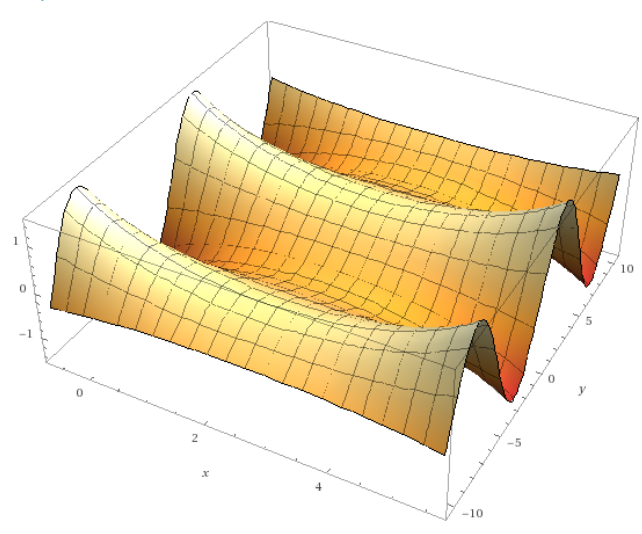
\includegraphics[width=0.7\linewidth]{3_1.png}\\
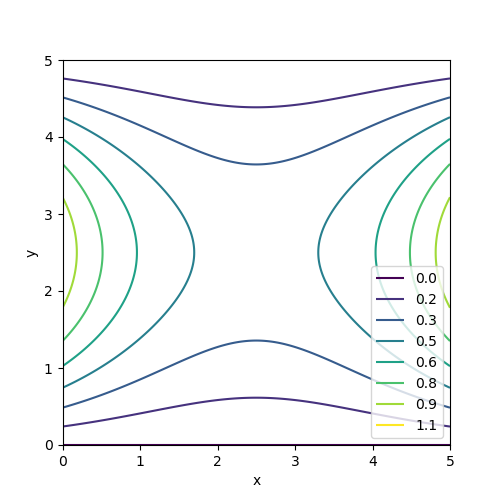
\includegraphics[width=0.7\linewidth]{3_2.png}

\pagebreak